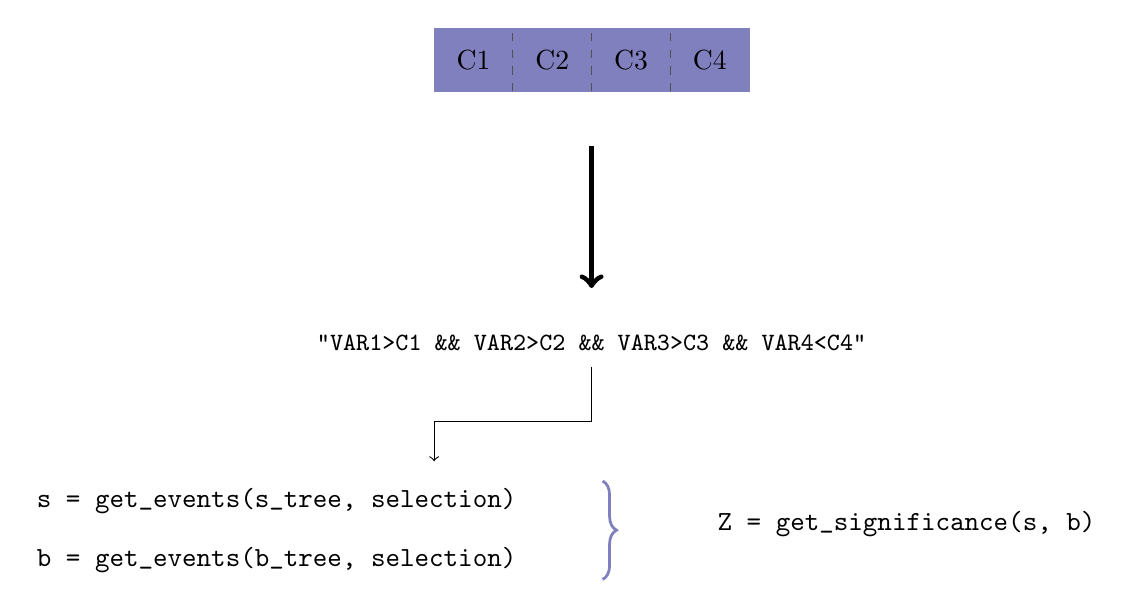
\begin{tikzpicture}
    \colorlet{c1}{blue!50!black!50}
    \colorlet{c2}{red!50!black!50}
    \colorlet{gray}{gray!40!black!80}

    \draw[c1, fill] (0,0.2) rectangle (4,1);

    \draw node at (0.5, 0.6) {C1};
    \draw node at (1.5, 0.6) {C2};
    \draw node at (2.5, 0.6) {C3};
    \draw node at (3.5, 0.6) {C4};

    \foreach \x in {1,2,3} \draw[dashed,gray] (\x,0.2) -- (\x,1);

    \draw[->,line width=2] (2,-0.5) -- (2,-2.3);

    \draw node at (2, -3) {\small \verb|"VAR1>C1 && VAR2>C2 && VAR3>C3 && VAR4<C4"|};

    \draw node at (-2,-5) {\verb|s = get_events(s_tree, selection)|};
    \draw node at (-2,-5.75) {\verb|b = get_events(b_tree, selection)|};

    \draw node at (6, -5.3) {\verb|Z = get_significance(s, b)|};

    \draw [decorate,decoration={brace,amplitude=5pt,mirror,raise=4pt},yshift=0pt,c1,line width=1]
(2,-6) -- (2,-4.75);

    \draw[->] (2,-3.3) |- (0,-4) -| (0,-4.5);

\end{tikzpicture}
